\subsection{Hyper-parameter tuning}
Just like it was possible to automatically search the hyper-parameter space for good tuning parameters in the classification setting, it is possible in the function estimation case. 


\begin{figure}
\centering
% This file was created by matlab2tikz.
% Minimal pgfplots version: 1.3
%
%The latest updates can be retrieved from
%  http://www.mathworks.com/matlabcentral/fileexchange/22022-matlab2tikz
%where you can also make suggestions and rate matlab2tikz.
%
\documentclass[tikz]{standalone}
\usepackage{pgfplots}
\usepackage{grffile}
\pgfplotsset{compat=newest}
\usetikzlibrary{plotmarks}
\usepackage{amsmath}

\begin{document}
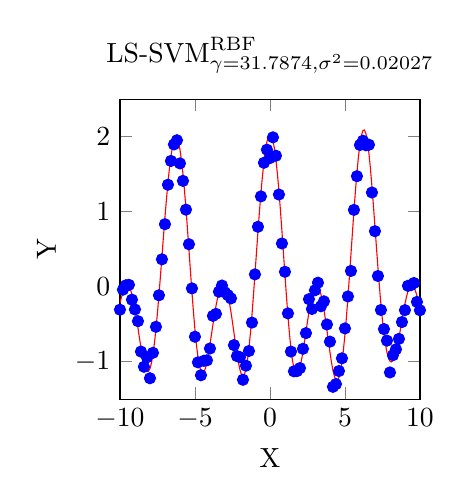
\begin{tikzpicture}

\begin{axis}[%
width=1.5in,
height=1.5in,
scale only axis,
xmin=-10,
xmax=10,
xlabel={X},
ymin=-1.5,
ymax=2.5,
ylabel={Y},
title={$\text{LS-SVM}_{\gamma\text{=31.7874,}\sigma{}^\text{2}\text{=0.02027}}^{\text{RBF}}$}
]
\addplot [color=red,solid,forget plot]
  table[row sep=crcr]{%
-10	-0.213262761564271\\
-9.9	-0.142478591462586\\
-9.8	-0.0793448278600375\\
-9.7	-0.0290871299652287\\
-9.6	0.00354128627906709\\
-9.5	0.0146389231847516\\
-9.4	0.0014854442796632\\
-9.3	-0.0372068057317912\\
-9.2	-0.101139578126474\\
-9.1	-0.188384754784025\\
-9	-0.295450732940575\\
-8.9	-0.417451111552073\\
-8.8	-0.54836015761066\\
-8.7	-0.681334313311297\\
-8.6	-0.809076237391692\\
-8.5	-0.924217391705701\\
-8.4	-1.01969655619064\\
-8.3	-1.0891143088334\\
-8.2	-1.12704685556991\\
-8.1	-1.12930614622694\\
-8	-1.0931366396388\\
-7.9	-1.01734224738166\\
-7.8	-0.902339926115156\\
-7.7	-0.750139254299917\\
-7.6	-0.564250307417169\\
-7.5	-0.349525371771638\\
-7.4	-0.111943512746484\\
-7.3	0.141649446458759\\
-7.2	0.403829761333681\\
-7.1	0.666895294241502\\
-7	0.923156741856179\\
-6.9	1.16520271391615\\
-6.8	1.38612426199147\\
-6.7	1.57969009939048\\
-6.6	1.74047099768306\\
-6.5	1.86391961687912\\
-6.4	1.94641889960253\\
-6.3	1.98531660850333\\
-6.2	1.97896431730091\\
-6.1	1.92677546758146\\
-6	1.82930912405298\\
-5.9	1.68837493150389\\
-5.8	1.50714251968933\\
-5.7	1.29022781256321\\
-5.6	1.04372203972044\\
-5.5	0.775128863897808\\
-5.4	0.493182006037289\\
-5.3	0.207529715069586\\
-5.2	-0.071708469581301\\
-5.1	-0.334486097297755\\
-5	-0.571429448456664\\
-4.9	-0.774432825918838\\
-4.8	-0.937184670987546\\
-4.7	-1.0555644603051\\
-4.6	-1.12786474973692\\
-4.5	-1.15481458840091\\
-4.4	-1.1394062281282\\
-4.3	-1.08655226706847\\
-4.2	-1.00262086443906\\
-4.1	-0.894909135000068\\
-4	-0.771117488512349\\
-3.9	-0.638880545664861\\
-3.8	-0.505395098113482\\
-3.7	-0.377165472976204\\
-3.6	-0.25986538284936\\
-3.5	-0.15829661720152\\
-3.4	-0.076411771861751\\
-3.3	-0.0173624363293186\\
-3.2	0.0164637355722698\\
-3.1	0.0234448149594588\\
-3	0.00277935713259821\\
-2.9	-0.0454075474076457\\
-2.8	-0.119923772719122\\
-2.7	-0.2183641248049\\
-2.6	-0.336994853900915\\
-2.5	-0.470706035278767\\
-2.4	-0.613064335527356\\
-2.3	-0.756488469166245\\
-2.2	-0.892555322646579\\
-2.1	-1.01242803698707\\
-2	-1.10738034141795\\
-1.9	-1.16937626873803\\
-1.8	-1.19165312213254\\
-1.7	-1.16924996613922\\
-1.6	-1.09942520913916\\
-1.5	-0.981915488238706\\
-1.4	-0.819003554392686\\
-1.3	-0.615383630150048\\
-1.2	-0.377836240340386\\
-1.1	-0.114747552622217\\
-1	0.164472689812005\\
-0.9	0.450008676734924\\
-0.799999999999999	0.732223019284894\\
-0.699999999999999	1.00214743291159\\
-0.6	1.25183573335143\\
-0.5	1.4745587727785\\
-0.399999999999999	1.66484713941422\\
-0.299999999999999	1.81841179086765\\
-0.199999999999999	1.9319909725078\\
-0.0999999999999996	2.00318052340469\\
0	2.03030243327841\\
0.0999999999999996	2.01235375272024\\
0.199999999999999	1.9490571002878\\
0.299999999999999	1.84100897769933\\
0.399999999999999	1.68989757532998\\
0.5	1.49874227573526\\
0.6	1.27209623402352\\
0.699999999999999	1.01615323295254\\
0.799999999999999	0.738710578626992\\
0.9	0.448959362048358\\
1	0.157098712729086\\
1.1	-0.126202428525651\\
1.2	-0.39044831118337\\
1.3	-0.625998791179181\\
1.4	-0.824717390134193\\
1.5	-0.980513307168073\\
1.6	-1.08971791571495\\
1.7	-1.1512567825635\\
1.8	-1.16660396654407\\
1.9	-1.13953247696962\\
2	-1.07569929730269\\
2.1	-0.982121710256422\\
2.2	-0.866611146612672\\
2.3	-0.737230143216886\\
2.4	-0.601827564140509\\
2.5	-0.467688940360609\\
2.6	-0.341315873120573\\
2.7	-0.228324993343533\\
2.8	-0.133437165178842\\
2.9	-0.060515022395779\\
3	-0.0126037695411765\\
3.1	0.00806308650816608\\
3.2	0.000116272064347903\\
3.3	-0.0368356050941697\\
3.4	-0.102049718523326\\
3.5	-0.193486050118584\\
3.6	-0.307683942198122\\
3.7	-0.439724546268655\\
3.8	-0.583315519240117\\
3.9	-0.731015883150585\\
4	-0.874595734026874\\
4.1	-1.00550212743108\\
4.2	-1.11538370966229\\
4.3	-1.19661627704551\\
4.4	-1.2427714403565\\
4.5	-1.24898077212411\\
4.6	-1.2121659244801\\
4.7	-1.13112733482442\\
4.8	-1.00650567509119\\
4.9	-0.840646828572783\\
5	-0.637409792058949\\
5.1	-0.401956242950502\\
5.2	-0.140551377926988\\
5.3	0.139609372295335\\
5.4	0.430550229711158\\
5.5	0.723659079426593\\
5.6	1.00985257446882\\
5.7	1.27979089273586\\
5.8	1.52416389161494\\
5.9	1.73405645184522\\
6	1.90138246596415\\
6.1	2.01935789597182\\
6.2	2.0829674870494\\
6.3	2.08937042591654\\
6.4	2.03818966147804\\
6.5	1.93163839679352\\
6.6	1.77445438508569\\
6.7	1.57363560131742\\
6.8	1.33799604082844\\
6.9	1.07758379403096\\
7	0.803021370673836\\
7.1	0.52483758664266\\
7.2	0.252859647769602\\
7.3	-0.00427651495553931\\
7.4	-0.239458330216288\\
7.5	-0.447255531456874\\
7.6	-0.623915292766853\\
7.7	-0.76722483255608\\
7.8	-0.876288257145369\\
7.9	-0.951271114914958\\
8	-0.993163247560142\\
8.1	-1.00359895046241\\
8.2	-0.984755579630112\\
8.3	-0.939331013226149\\
8.4	-0.870580666246955\\
8.5	-0.782379680020918\\
8.6	-0.679268179278144\\
8.7	-0.56643846074942\\
8.8	-0.449632419326794\\
8.9	-0.334933684198312\\
9	-0.228458894122546\\
9.1	-0.135972700243537\\
9.2	-0.0624678446152139\\
9.3	-0.0117620385539706\\
9.4	0.013834497549275\\
9.5	0.0137334936510258\\
9.6	-0.010868124858183\\
9.7	-0.0570900080219115\\
9.8	-0.120627416327316\\
9.9	-0.196139480243158\\
10	-0.277722702248705\\
};
\addplot [color=blue,only marks,mark=*,mark options={solid},forget plot]
  table[row sep=crcr]{%
-10	-0.306579133527982\\
-9.8	-0.0397382555553657\\
-9.6	0.018739660609576\\
-9.4	0.0242905480075732\\
-9.2	-0.173380769716921\\
-9	-0.303452947386662\\
-8.8	-0.459547263627656\\
-8.6	-0.865085860768563\\
-8.4	-1.06784448545167\\
-8.2	-0.941742958419704\\
-8	-1.22066061822186\\
-7.8	-0.881877827486431\\
-7.6	-0.534964538044644\\
-7.4	-0.114653722995193\\
-7.2	0.365063866304641\\
-7	0.833183768477336\\
-6.8	1.3593888028889\\
-6.6	1.6764672224338\\
-6.4	1.89657728080095\\
-6.2	1.95242004354036\\
-6	1.64392823759623\\
-5.8	1.41069727246189\\
-5.6	1.02715004301935\\
-5.4	0.566008817029371\\
-5.2	-0.0226588916021791\\
-5	-0.667002890632711\\
-4.8	-1.00885127695319\\
-4.6	-1.18052735154478\\
-4.4	-0.987745467811725\\
-4.2	-0.982006760185838\\
-4	-0.82409491495306\\
-3.8	-0.389406083461653\\
-3.6	-0.362798054582325\\
-3.4	-0.0668089334738737\\
-3.2	0.0152031165919985\\
-3	-0.0756469343852673\\
-2.8	-0.112338464968575\\
-2.6	-0.156181529203947\\
-2.4	-0.77899329546166\\
-2.2	-0.924930542321883\\
-2	-0.939996483241433\\
-1.8	-1.24123176786791\\
-1.6	-1.05325139523663\\
-1.4	-0.857442817230265\\
-1.2	-0.47867949734374\\
-1	0.164137461033253\\
-0.799999999999999	0.798528324906496\\
-0.6	1.20425025884851\\
-0.399999999999999	1.65189112389713\\
-0.199999999999999	1.82666452394961\\
0	1.71497122229152\\
0.199999999999999	1.99125121667456\\
0.399999999999999	1.74601395259658\\
0.6	1.22859304817884\\
0.799999999999999	0.576006043167302\\
1	0.198369702065894\\
1.2	-0.356093645541498\\
1.4	-0.864817391491114\\
1.6	-1.12859035792103\\
1.8	-1.12571135333162\\
2	-1.08541915281891\\
2.2	-0.828146555519386\\
2.4	-0.619062350438906\\
2.6	-0.166384116930707\\
2.8	-0.297194787264751\\
3	-0.0483218061484544\\
3.2	0.053009933786154\\
3.4	-0.260413518102873\\
3.6	-0.195231272475295\\
3.8	-0.503916733277877\\
4	-0.732599750127662\\
4.2	-1.33524884529104\\
4.4	-1.2985987129247\\
4.6	-1.12472571614096\\
4.8	-0.954881987385641\\
5	-0.556407122309299\\
5.2	-0.130055763458628\\
5.4	0.209937041851235\\
5.6	1.02393741156959\\
5.8	1.47338319728387\\
6	1.88951982345171\\
6.2	1.94540993806249\\
6.4	1.88609300482996\\
6.6	1.89243215815344\\
6.8	1.25572426230034\\
7	0.740131583568841\\
7.2	0.14248777755351\\
7.4	-0.310578825334796\\
7.6	-0.565333766918074\\
7.8	-0.719470674351168\\
8	-1.14341280005323\\
8.2	-0.913369219359977\\
8.4	-0.835654817371107\\
8.6	-0.695767150416593\\
8.8	-0.471530820082818\\
9	-0.31262727143036\\
9.2	0.0114268286448022\\
9.4	0.0205720531660902\\
9.6	0.0490609089602083\\
9.8	-0.20311160964176\\
10	-0.314123795052465\\
};
\end{axis}
\end{tikzpicture}%
\end{document}
% This file was created by matlab2tikz.
% Minimal pgfplots version: 1.3
%
%The latest updates can be retrieved from
%  http://www.mathworks.com/matlabcentral/fileexchange/22022-matlab2tikz
%where you can also make suggestions and rate matlab2tikz.
%
\documentclass[tikz]{standalone}
\usepackage{pgfplots}
\usepackage{grffile}
\pgfplotsset{compat=newest}
\usetikzlibrary{plotmarks}
\usepackage{amsmath}

\begin{document}
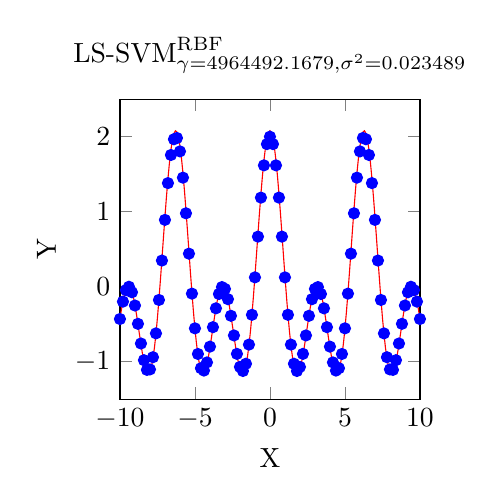
\begin{tikzpicture}

\begin{axis}[%
width=1.5in,
height=1.5in,
scale only axis,
xmin=-10,
xmax=10,
xlabel={X},
ymin=-1.5,
ymax=2.5,
ylabel={Y},
title={$\text{LS-SVM}_{\gamma\text{=4964492.1679,}\sigma{}^\text{2}\text{=0.023489}}^{\text{RBF}}$}
]
\addplot [color=red,solid,forget plot]
  table[row sep=crcr]{%
-10	-0.431331782639043\\
-9.9	-0.304119166472711\\
-9.8	-0.191764312900384\\
-9.7	-0.0999102841381132\\
-9.6	-0.0331842847589969\\
-9.5	0.00504946253817296\\
-9.4	0.012861876382152\\
-9.3	-0.0101466813382787\\
-9.2	-0.0628280477788594\\
-9.1	-0.142538739660447\\
-9	-0.245256401029012\\
-8.9	-0.365752546049465\\
-8.8	-0.497813526340048\\
-8.7	-0.634501184798639\\
-8.6	-0.768443863046565\\
-8.5	-0.892147308877627\\
-8.4	-0.998313805246278\\
-8.3	-1.08015685057651\\
-8.2	-1.13169829240203\\
-8.1	-1.14803517031083\\
-8	-1.12556471053985\\
-7.9	-1.06215782022146\\
-7.8	-0.957273832176739\\
-7.7	-0.81201189568464\\
-7.6	-0.629097078190218\\
-7.5	-0.412801800442894\\
-7.4	-0.168805619854606\\
-7.3	0.0960013950259457\\
-7.2	0.373764380798885\\
-7.1	0.6559492644935\\
-7	0.933657331029236\\
-6.9	1.19795656859519\\
-6.8	1.44021674017233\\
-6.7	1.65243485192024\\
-6.6	1.82753802941059\\
-6.5	1.959651753909\\
-6.4	2.04432287859189\\
-6.3	2.07868872880872\\
-6.2	2.06158577264405\\
-6.1	1.99359372214666\\
-6	1.87701340737194\\
-5.9	1.71577928799996\\
-5.8	1.51530996863337\\
-5.7	1.28230249290382\\
-5.6	1.0244784207661\\
-5.5	0.750291641419973\\
-5.4	0.468609437480446\\
-5.3	0.188379404656003\\
-5.2	-0.0817046153707543\\
-5.1	-0.333524436300959\\
-5	-0.559834660222095\\
-4.9	-0.754523491309057\\
-4.8	-0.912827171115857\\
-4.7	-1.03148983877496\\
-4.6	-1.10886278040785\\
-4.5	-1.14493941776539\\
-4.4	-1.14132491764175\\
-4.3	-1.10114189306176\\
-4.2	-1.02887621633861\\
-4.1	-0.930169366931768\\
-4	-0.811565887118153\\
-3.9	-0.680226318078802\\
-3.8	-0.543617358093292\\
-3.7	-0.409191867024891\\
-3.6	-0.284071707155647\\
-3.5	-0.174746254165592\\
-3.4	-0.0867987488032177\\
-3.3	-0.024671521266446\\
-3.2	0.00852044813269814\\
-3.1	0.0111201088895021\\
-3	-0.0170022205456315\\
-2.9	-0.0744433763276647\\
-2.8	-0.158326075992265\\
-2.7	-0.264419490065749\\
-2.6	-0.387316792045654\\
-2.5	-0.520662508569691\\
-2.4	-0.657420472644552\\
-2.3	-0.790171538601403\\
-2.2	-0.911429012075913\\
-2.1	-1.01395902648628\\
-2	-1.09109288440788\\
-1.9	-1.13701868417562\\
-1.8	-1.14704035686444\\
-1.7	-1.11779351634068\\
-1.6	-1.04740922739445\\
-1.5	-0.935618858970764\\
-1.4	-0.783795530564684\\
-1.3	-0.594930186503793\\
-1.2	-0.373542942908067\\
-1.1	-0.125532939456135\\
-1	0.142027612253058\\
-0.9	0.421147258913771\\
-0.799999999999999	0.703207171854714\\
-0.699999999999999	0.979279680268011\\
-0.6	1.24046102567082\\
-0.5	1.4782053078104\\
-0.399999999999999	1.68464652333176\\
-0.299999999999999	1.8528960480538\\
-0.199999999999999	1.97730386471602\\
-0.0999999999999996	2.05367325385993\\
0	2.07942049074634\\
0.0999999999999996	2.05367325385993\\
0.199999999999999	1.97730386471602\\
0.299999999999999	1.8528960480538\\
0.399999999999999	1.68464652333176\\
0.5	1.4782053078104\\
0.6	1.24046102567082\\
0.699999999999999	0.979279680268011\\
0.799999999999999	0.703207171854715\\
0.9	0.421147258913772\\
1	0.142027612253058\\
1.1	-0.125532939456135\\
1.2	-0.373542942908067\\
1.3	-0.594930186503793\\
1.4	-0.783795530564684\\
1.5	-0.935618858970764\\
1.6	-1.04740922739445\\
1.7	-1.11779351634068\\
1.8	-1.14704035686443\\
1.9	-1.13701868417562\\
2	-1.09109288440788\\
2.1	-1.01395902648628\\
2.2	-0.911429012075912\\
2.3	-0.790171538601403\\
2.4	-0.657420472644552\\
2.5	-0.520662508569692\\
2.6	-0.387316792045656\\
2.7	-0.264419490065749\\
2.8	-0.158326075992265\\
2.9	-0.0744433763276649\\
3	-0.017002220545631\\
3.1	0.0111201088895025\\
3.2	0.00852044813269881\\
3.3	-0.0246715212664457\\
3.4	-0.0867987488032185\\
3.5	-0.174746254165593\\
3.6	-0.284071707155648\\
3.7	-0.409191867024892\\
3.8	-0.543617358093293\\
3.9	-0.680226318078801\\
4	-0.811565887118153\\
4.1	-0.930169366931767\\
4.2	-1.02887621633861\\
4.3	-1.10114189306176\\
4.4	-1.14132491764175\\
4.5	-1.14493941776539\\
4.6	-1.10886278040785\\
4.7	-1.03148983877496\\
4.8	-0.912827171115855\\
4.9	-0.754523491309055\\
5	-0.559834660222093\\
5.1	-0.333524436300956\\
5.2	-0.0817046153707526\\
5.3	0.188379404656005\\
5.4	0.468609437480447\\
5.5	0.75029164141997\\
5.6	1.0244784207661\\
5.7	1.28230249290381\\
5.8	1.51530996863338\\
5.9	1.71577928799997\\
6	1.87701340737195\\
6.1	1.99359372214667\\
6.2	2.06158577264406\\
6.3	2.07868872880873\\
6.4	2.04432287859189\\
6.5	1.959651753909\\
6.6	1.82753802941059\\
6.7	1.65243485192024\\
6.8	1.44021674017233\\
6.9	1.19795656859519\\
7	0.933657331029237\\
7.1	0.6559492644935\\
7.2	0.37376438079889\\
7.3	0.0960013950259471\\
7.4	-0.16880561985461\\
7.5	-0.412801800442904\\
7.6	-0.629097078190218\\
7.7	-0.812011895684628\\
7.8	-0.957273832176735\\
7.9	-1.06215782022144\\
8	-1.12556471053984\\
8.1	-1.14803517031082\\
8.2	-1.13169829240202\\
8.3	-1.08015685057649\\
8.4	-0.998313805246246\\
8.5	-0.89214730887763\\
8.6	-0.768443863046565\\
8.7	-0.634501184798624\\
8.8	-0.497813526340026\\
8.9	-0.365752546049458\\
9	-0.245256401028998\\
9.1	-0.142538739660397\\
9.2	-0.0628280477788452\\
9.3	-0.010146681338236\\
9.4	0.012861876382152\\
9.5	0.00504946253817296\\
9.6	-0.0331842847589685\\
9.7	-0.099910284138099\\
9.8	-0.191764312900369\\
9.9	-0.304119166472697\\
10	-0.431331782639015\\
};
\addplot [color=blue,only marks,mark=*,mark options={solid},forget plot]
  table[row sep=crcr]{%
-10	-0.43098946726306\\
-9.8	-0.199040176459257\\
-9.6	-0.0454675090972562\\
-9.4	-0.000920685447996283\\
-9.2	-0.0742034490193951\\
-9	-0.250813553640597\\
-8.8	-0.495349259142413\\
-8.6	-0.757398242051853\\
-8.4	-0.979967241528048\\
-8.2	-1.10910282152591\\
-8	-1.103159514132\\
-7.8	-0.940222204621165\\
-7.6	-0.622477140428825\\
-7.4	-0.17680515538033\\
-7.2	0.348533958318501\\
-7	0.890639472551138\\
-6.8	1.38110148280297\\
-6.6	1.75611654959898\\
-6.4	1.96601748445563\\
-6.2	1.98273439930208\\
-6	1.80402424538286\\
-5.8	1.45380914670929\\
-5.6	0.978570742329\\
-5.4	0.440362969487297\\
-5.2	-0.0924675861268539\\
-5	-0.555409343613226\\
-4.8	-0.897188872354681\\
-4.6	-1.08699614833922\\
-4.4	-1.11842588404008\\
-4.2	-1.00954947545738\\
-4	-0.799143654672225\\
-3.8	-0.539707869332161\\
-3.6	-0.288407101801892\\
-3.4	-0.0974007022296354\\
-3.2	-0.00510985703656031\\
-3	-0.0298222099500793\\
-2.8	-0.166656462158408\\
-2.6	-0.388372082068571\\
-2.4	-0.6498947321018\\
-2.2	-0.895833987233766\\
-2	-1.06979045741075\\
-1.8	-1.12396051102723\\
-1.6	-1.02749429809604\\
-1.4	-0.772255197768418\\
-1.2	-0.37503596106457\\
-1	0.124155469320997\\
-0.799999999999999	0.66750718704588\\
-0.6	1.18769336938635\\
-0.399999999999999	1.61776770335005\\
-0.199999999999999	1.90112757184413\\
0	2\\
0.199999999999999	1.90112757184413\\
0.399999999999999	1.61776770335005\\
0.6	1.18769336938635\\
0.799999999999999	0.66750718704588\\
1	0.124155469320997\\
1.2	-0.37503596106457\\
1.4	-0.772255197768418\\
1.6	-1.02749429809604\\
1.8	-1.12396051102723\\
2	-1.06979045741075\\
2.2	-0.895833987233766\\
2.4	-0.6498947321018\\
2.6	-0.388372082068571\\
2.8	-0.166656462158408\\
3	-0.0298222099500793\\
3.2	-0.00510985703656031\\
3.4	-0.0974007022296354\\
3.6	-0.288407101801892\\
3.8	-0.539707869332161\\
4	-0.799143654672225\\
4.2	-1.00954947545738\\
4.4	-1.11842588404008\\
4.6	-1.08699614833922\\
4.8	-0.897188872354681\\
5	-0.555409343613226\\
5.2	-0.0924675861268539\\
5.4	0.440362969487297\\
5.6	0.978570742329\\
5.8	1.45380914670929\\
6	1.80402424538286\\
6.2	1.98273439930208\\
6.4	1.96601748445563\\
6.6	1.75611654959898\\
6.8	1.38110148280297\\
7	0.890639472551138\\
7.2	0.348533958318501\\
7.4	-0.17680515538033\\
7.6	-0.622477140428825\\
7.8	-0.940222204621165\\
8	-1.103159514132\\
8.2	-1.10910282152591\\
8.4	-0.979967241528048\\
8.6	-0.757398242051853\\
8.8	-0.495349259142413\\
9	-0.250813553640597\\
9.2	-0.0742034490193951\\
9.4	-0.000920685447996283\\
9.6	-0.0454675090972562\\
9.8	-0.199040176459257\\
10	-0.43098946726306\\
};
\end{axis}
\end{tikzpicture}%
\end{document}
\caption{Exemplary tuning results on noise free and noisy data.}
\label{fig:autoTune}
\end{figure}

\subsection{The Bayesian Framework}

\subsection{Robust Regression}
